\documentclass{beamer}
\usetheme{metropolis}
\usepackage{graphicx}
\usepackage{subfig}
\usepackage{hyperref}
\title{Algebra-Based Physics-1: Mechanics (PHYS135A-01): Week 3}
\date{September 18th - September 22nd, 2017}
\author{Jordan Hanson}
\institute{Whittier College Department of Physics and Astronomy}

\begin{document}
\maketitle

\section{Week 2 Review}

\begin{frame}{Week 2 Review}
\begin{enumerate}
\item Displacement, average velocity and acceleration
\begin{itemize}
\item \textit{Mathematics review}: slope of a function
\end{itemize}
\item The case of constant acceleration
\begin{itemize}
\item An \textit{an equation of motion} for constant acceleration
\item Derivation of \alert{common equations of motion}
\item Average quantities and exercises
\end{itemize}
\item \textbf{Lab Activity: Measuring acceleration of gravity: \textit{g}}
\item Exercises with vectors, graphs, and equations of motion
\end{enumerate}
\end{frame}

\section{Week 2 Review Problems}

\begin{frame}{Week 2 Review Problems}
\small
\begin{minipage}[b]{0.45\linewidth}
If a subway train is moving to the left (has a negative velocity) and then comes to a stop, what is the direction of its acceleration? Is the acceleration positive or negative?
\begin{itemize}
\vspace{0.5cm}
\item A: To the right, positive
\item B: To the right, negative
\item C: To the left, positive
\item D: To the left, negative
\end{itemize}
\end{minipage}
\hspace{0.5cm}
\begin{minipage}[b]{0.45\linewidth}
An object that is thrown straight up falls back to Earth.  When is its velocity zero?  Does its velocity change direction?  Does the acceleration change sign?
\begin{itemize}
\item A: During flight, yes, no
\item B: At the peak height, yes, yes
\item C: At the peak height, yes, no
\item D: During flight, no, no
\end{itemize}
\end{minipage}
\end{frame}

\section{Week 3 Summary}

\begin{frame}{Week 3 Summary}
\begin{enumerate}
\item Working with vectors: displacement, velocity and acceleration
\begin{itemize}
\item Breaking into components, graphical methods
\item Analytical methods
\item \textbf{Lab-activity: measuring different accelerations}
\item \textbf{Lab-activity: testing component independence}
\end{itemize}
\item Combining free-fall and vector components: \alert{projectile motion}
\item Relative motion and addition of velocities
\end{enumerate}
\end{frame}

\section{Working with vectors: displacement, velocity and acceleration}

\begin{frame}{Working with vectors: displacement, velocity and acceleration}
In general, the displacement of an object depends on time:
\begin{equation}
\vec{r}(t) = x(t) \hat{i} + y(t) \hat{j} + z(t) \hat{k}
\end{equation}
\begin{itemize}
\item $x(t)$ is the displacement in the x-direction
\item $y(t)$ is the displacement in the y-direction
\item $z(t)$ is the displacement in the z-direction
\end{itemize}
\end{frame}

\begin{frame}{Working with vectors: displacement, velocity and acceleration}
\begin{figure}
\centering
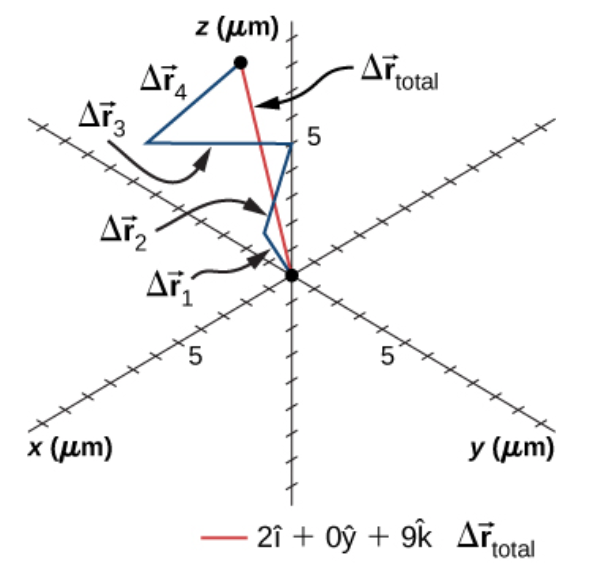
\includegraphics[width=0.6\textwidth,trim=0cm 2cm 0cm 0cm,clip=true]{figures/Brownian.png}
\caption{\label{fig:brown} An example of a displacement vector at different moments in time.}
\end{figure}
\end{frame}

\begin{frame}{Working with vectors: displacement, velocity and acceleration}
The particle in Fig. \ref{fig:brown} has four displacement vectors at four moments in time:
\begin{itemize}
\item $\vec{r}_{\rm 1} = 2.0\hat{i} + 1.0\hat{j} + 3.0\hat{k}\quad(\mu m)$ at $t_{\rm 1}$
\item $\vec{r}_{\rm 2} = -1.0\hat{i} + 0.0\hat{j} + 3.0\hat{k}\quad(\mu m)$ at $t_{\rm 2}$
\item $\vec{r}_{\rm 3} = 4.0\hat{i} + -2.0\hat{j} + 1.0\hat{k}\quad(\mu m)$ at $t_{\rm 3}$
\item $\vec{r}_{\rm 4} = -3.0\hat{i} + 1.0\hat{j} + 2.0\hat{k}\quad(\mu m)$ at $t_{\rm 4}$
\end{itemize}
What is the total displacement of the particle from the origin?
\end{frame}

\begin{frame}{Working with vectors: displacement, velocity and acceleration}
We can think of this type of problem as an accounting problem, lining up columns (units: $\mu m$):
\begin{figure}
\begin{tabular}{| c | c | c | c | c |}
\hline
$t_{\rm i}$ & $\vec{r}_{\rm i}(t_{\rm i})$ & $x(t_{\rm i})$ & $y(t_{\rm i})$ & $y(t_{\rm i})$ \\
\hline
$t_{\rm 1}$ & $\vec{r}_{\rm 1}(t_{\rm 1})$ & 2.0 & 1.0 & 3.0 \\
\hline
$t_{\rm 2}$ & $\vec{r}_{\rm 2}(t_{\rm 2})$ & -1.0 & 0.0 & 3.0 \\
\hline
$t_{\rm 3}$ & $\vec{r}_{\rm 3}(t_{\rm 3})$ & 4.0 & -2.0 & 1.0 \\
\hline
$t_{\rm 4}$ & $\vec{r}_{\rm 4}(t_{\rm 4})$ & -3.0 & 1.0 & 2.0 \\
\hline
\hline
$t_{\rm total}$ & $\vec{r}_{\rm total}(t_{\rm total})$ & 2.0 & 0.0 & 9.0 \\
\hline
\end{tabular}
\caption{\label{tab:account} Accounting for the different displacement components, in units of $\mu m$.}
\end{figure}
\end{frame}

\begin{frame}{Working with vectors: displacement, velocity and acceleration}
\begin{figure}
\centering
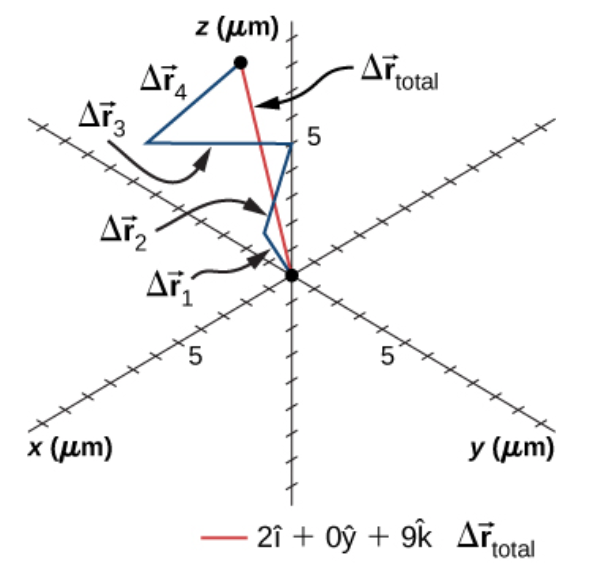
\includegraphics[width=0.6\textwidth]{figures/Brownian.png}
\caption{\label{fig:brown2} The total displacement of the particle is $\vec{r}_{\rm total} = 2.0\hat{i} + 0.0\hat{k} + 9.0\hat{k}\quad (\mu m)$.}
\end{figure}
\end{frame}

\begin{frame}{Working with vectors: displacement, velocity and acceleration}
\small
The 18th hole at Pebble Beach Golf Course is a dogleg to the left of length 496.0 meters.  The fairway off the tee is taken to be the x direction.  A golfer hits his tee shot a distance of 300 meters, corresponding to a displacement of $\vec{r}_{\rm 1} = 300.0 \hat{i} \quad (m)$, and then hits a second shot 189.0 meters with $\vec{r}_{\rm 2} = 150.0 \hat{i} + 80.0 \hat{j} \quad m$.  What is the final displacement from the tee?
\begin{itemize}
\item A: $\vec{r}_{\rm final} = 150.0 \hat{i} + 80.0\hat{j}\quad (m)$
\item B: $\vec{r}_{\rm final} = 450.0 \hat{i} + 230.0\hat{j}\quad (m)$
\item C: $\vec{r}_{\rm final} = 230.0 \hat{i} + 0.0\hat{j}\quad (m)$
\item D: $\vec{r}_{\rm final} = 450.0 \hat{i} + 80.0\hat{j}\quad (m)$
\end{itemize}
\end{frame}

\begin{frame}{Working with vectors: displacement, velocity and acceleration}
\small
If the first shot takes 5.0 seconds, the second shot takes 4.0 seconds, and the walking time in between the shots is 60.0 seconds, what is the average velocity vector for the ball after the two shots?
\begin{itemize}
\item A: $\vec{r}_{\rm final} = 50.7 \hat{i} + 11.6\hat{j}\quad (m/s)$
\item B: $\vec{v}_{\rm final} = 17.0 \hat{i} + 80.3\hat{j}\quad (m/s)$
\item C: $\vec{v}_{\rm final} = 6.5 \hat{i} + 1.2\hat{j}\quad (m)$
\item D: $\vec{v}_{\rm final} = 6.5 \hat{i} + 1.2\hat{j}\quad (m/s)$
\end{itemize}
\end{frame}

\begin{frame}{Working with vectors: displacement, velocity and acceleration}
The prior problem indicates something you may already have guessed:
\begin{equation}
\vec{v}_{\rm avg}(t) = v_{\rm x}(t) \hat{i} + v_{\rm y}(t) \hat{j} + v_{\rm z}(t) \hat{k} = \frac{\Delta\vec{r}}{\Delta t}
\label{eq:vel}
\end{equation}
\begin{itemize}
\item $v_{\rm x}(t)$ is the avg. velocity in the x-direction
\item $v_{\rm y}(t)$ is the avg. velocity in the y-direction
\item $v_{\rm z}(t)$ is the avg. velocity in the z-direction
\end{itemize}
In other words, we divide each displacement component by the time, to get a vector where each component is the average velocity in that direction.  $\Delta\vec{r} = \vec{r}_{\rm f} - \vec{r}_{\rm i}$.  These next problems help us practice breaking vectors into components.
\end{frame}

\begin{frame}{Working with vectors: displacement, velocity and acceleration}
A gamma ray is radiated from a radioactive source, and travels at the speed of light (0.3 m/ns) 60 degrees with respect to the x-axis, in the positive direction.  A detection screen is 1.0 to the right of the radioactive source.  When does the gamma ray hit the screen?
\begin{itemize}
\item A: $20/\sqrt{3}$ ns
\item B: $20/(3\sqrt{3})$ ns
\item C: $20/3$ ns
\item D: $10$ ns
\end{itemize}
\end{frame}

\begin{frame}{Working with vectors: displacement, velocity and acceleration}
A person changes lanes on a highway.  Her vehicle is traveling at 100 km/hr.  She turns the wheel so that the car's velocity points 20 degrees from the direction down the highway.  By what percentage must she increase her speed in order to maintain 100 km/hr \textit{down the highway}?
\begin{itemize}
\item A: 1\%
\item B: 2\%
\item C: 6\%
\item D: 10\%
\end{itemize}
\end{frame}

\begin{frame}{Working with vectors: displacement, velocity and acceleration}
A particle would travel with velocity of 4 m/s, 30 degrees above horizontal ($+\hat{i}$ direction), but the medium in which it moves has a velocity of 2 m/s, 225 degrees from the horizontal ($+\hat{i}$ direction).  To find the actual velocity of the particle, add the velocity vectors:
\begin{itemize}
\item A: $(2.45)\hat{i}-(0.38)\hat{j} \quad (m/s)$
\item B: $(1.45)\hat{i}+(0.38)\hat{j} \quad (m/s)$
\item C: $(-2.45)\hat{i}+(0.38)\hat{j} \quad (m/s)$
\item D: $(2.45)\hat{i}-(1.38)\hat{j} \quad (m/s)$
\end{itemize}
\end{frame}

\begin{frame}{Working with vectors: displacement, velocity and acceleration}
In the previous example we had to subtract vectors.  There are several approaches to doing this.  Consider two vectors $\vec{A}$ and $\vec{B}$.\\
\begin{itemize}
\item Break into components: $\vec{A}-\vec{B} = \hat{i}(A_x-B_x) + \hat{j}(A_y-B_y)$
\item Add the opposite: $\vec{A}-\vec{B} = \vec{A}+(-\vec{B})$ (flip one vector head to tail).
\item Rearrange equation: $\vec{C} = \vec{A}-\vec{B} \rightarrow \vec{A} = \vec{C}+\vec{B}$ (usually graphical).
\end{itemize}
\small (Note to self: draw example of each).
\end{frame}

\begin{frame}{Working with vectors: displacement, velocity and acceleration}
\begin{columns}[T]
\begin{column}{0.5\textwidth}
\small Suppose a paricle experiences a displacement equivalent to $\vec{R}-\vec{B}$.  What is the final position of the particle?  ($|R| = 5$ m, $|B| = 4$ m).
\begin{itemize}
\item A: $3\hat{i}$ m
\item B: $4\hat{i}$ m
\item C: $-3\hat{i}$ m
\item D: $-5\hat{i}$ m
\end{itemize}
\end{column}
\begin{column}{0.5\textwidth}
\begin{figure}
\centering
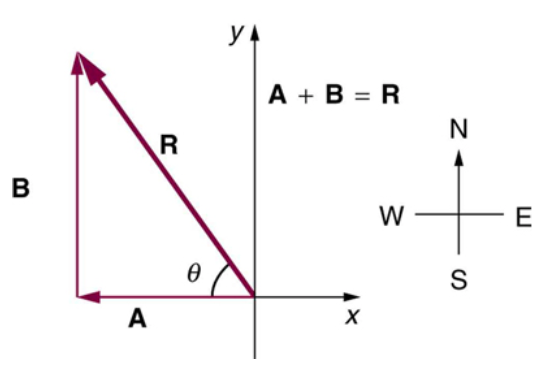
\includegraphics[width=0.9\textwidth]{figures/vecdiag.png}
\caption{\label{fig:vecdiag} The path of the particle.}
\end{figure}
\end{column}
\end{columns}
\end{frame}

\begin{frame}{Working with vectors: displacement, velocity and acceleration}
\begin{columns}[T]
\begin{column}{0.5\textwidth}
\small Two effects give a particle two velocity vectors: $\vec{v}_{\rm A}$ and $\vec{v}_{\rm B}$.  The total velocity is observed (see figure).  First, solve for $v_{\rm A}$, $v_{\rm B}$. (Hint: use the law of sines).
\begin{itemize}
\item A: 3.45 m/s, 3.94 m/s
\item B:  3.81 m/s, 3.2 m/s
\item C: 2.90 m/s, 4.51 m/s
\item D: 3.94 m/s, 3.45 m/s
\end{itemize}
\end{column}
\begin{column}{0.5\textwidth}
\begin{figure}
\centering
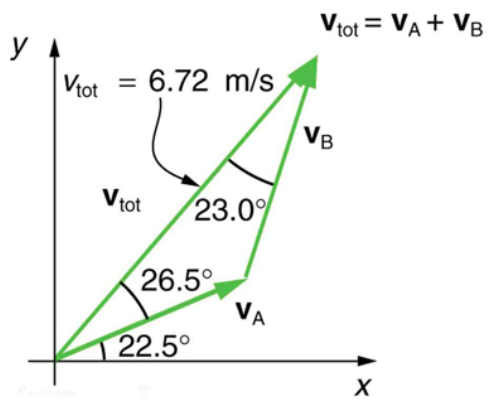
\includegraphics[width=0.9\textwidth]{figures/vecdiag2.png}
\caption{\label{fig:vecdiag2} The velocities of the particle.}
\end{figure}
\end{column}
\end{columns}
\end{frame}

\begin{frame}{Working with vectors: displacement, velocity and acceleration}
\begin{columns}[T]
\begin{column}{0.5\textwidth}
\small Solve for $\vec{v}_{\rm A}$.
\begin{itemize}
\item A: (2.19,2.32) m/s
\item B: (3.19,3.32) m/s
\item C: (3.19,1.32) m/s
\item D: (1.32,3.25) m/s
\end{itemize}
\end{column}
\begin{column}{0.5\textwidth}
\begin{figure}
\centering
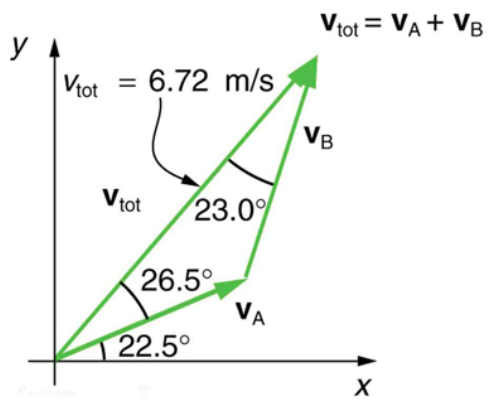
\includegraphics[width=0.9\textwidth]{figures/vecdiag2.png}
\caption{\label{fig:vecdiag3} The velocities of the particle.}
\end{figure}
\end{column}
\end{columns}
\end{frame}

\begin{frame}{Working with vectors: displacement, velocity and acceleration}
\begin{columns}[T]
\begin{column}{0.5\textwidth}
\small Solve for $\vec{v}_{\rm B}$ by using $\vec{v}_{\rm tot} - \vec{v}_{\rm A}$.
\begin{itemize}
\item A: (1.22,3.75)
\item B: (1.51,4.01)
\item C: (3.75,1.22)
\item D: (4.01,1.32)
\end{itemize}
\end{column}
\begin{column}{0.5\textwidth}
\begin{figure}
\centering
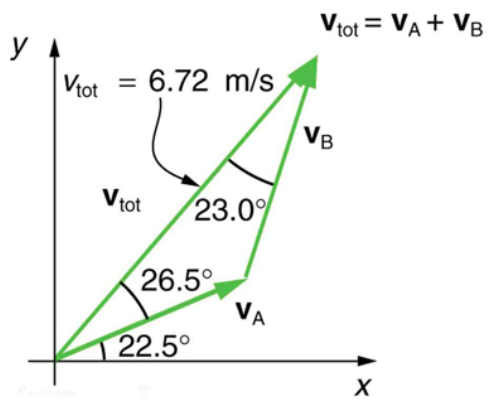
\includegraphics[width=0.9\textwidth]{figures/vecdiag2.png}
\caption{\label{fig:vecdiag4} The velocities of the particle.}
\end{figure}
\end{column}
\end{columns}
\end{frame}

\begin{frame}{Working with vectors: displacement, velocity and acceleration}
The following \textbf{lab activity} will provide practice for deriving kinematic quantities graphically.  Set up a ramp with a cart, and a motion detector on the bottom:
\begin{figure}
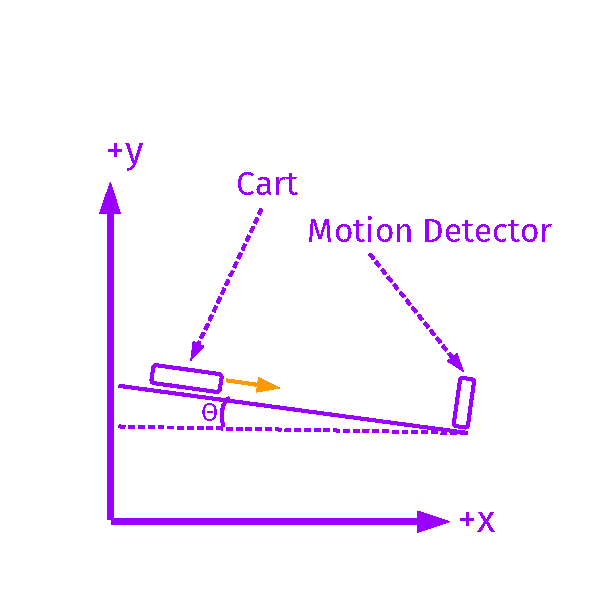
\includegraphics[width=0.6\textwidth,trim=0cm 1cm 0cm 2cm,clip=true]{figures/GraphAccel.pdf}
\caption{\label{fig:graphaccel} Cart with ramp and motion detector.}
\end{figure}
\end{frame}

\begin{frame}{Working with vectors: displacement, velocity and acceleration}
\begin{enumerate}
\item Once the setup is complete, release the cart and stop it, recording the position with LoggerPro.
\item Grab the cart before it hits the motion detector.
\item Record in your notebooks the position and velocity graphs; describe where the acceleration is constant in the data, and note whether it is positive or negative.
\item Repeat for a different value of $\theta$, the ramp incline angle.  Compare acceleration versus $\theta$ from the graphs.
\end{enumerate}
\end{frame}

\begin{frame}{Working with vectors: displacement, velocity and acceleration}
In the kinematic description of motion, \alert{\textit{we are able to treat the different components of motion separately.}}  In many cases, motion in the horizontal direction does not affect motion in the vertical direction, and vice versa.\\
\vspace{0.5cm}
\small
\framebox[1.1\width]{\textbf{Motions in displacement components are independent.}} \\
\vspace{1cm}
\textit{(Exception: non-conservative forces.  More on this later.)}
\end{frame}

\begin{frame}{Projectile motion}
\small
\begin{figure}
\centering
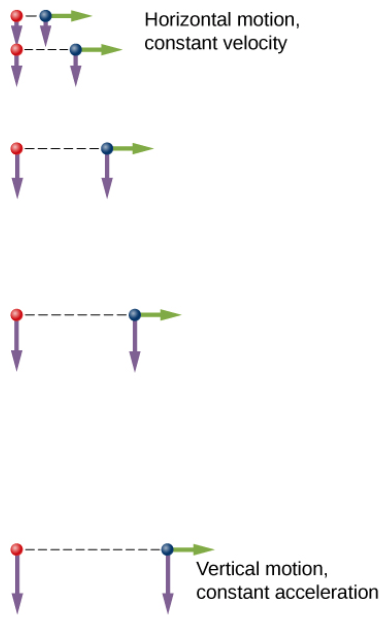
\includegraphics[width=0.4\textwidth]{figures/fall.png}
\caption{\label{fig:fall} Independence of motion in two dimensions.}
\end{figure}
\end{frame}

\begin{frame}{Projectile motion}
Is this true?  Figure \ref{fig:fall} is testable by experiment. \\
\vspace{0.5cm}
\small
Procedure:
\begin{enumerate}
\item Obtain two marbles, a meter stick, and a stopwatch.
\item Measure the height of the lab bench, $\Delta x$.
\item We are going to drop a marble from this height ($\Delta x$) and record the time.  Show first algebraically that the predicted time for the marble to fall is $t = \sqrt{2\Delta x/g}$.
\item Measure $t$ for several trials.  Does it match the expected result $\sqrt{2\Delta x/g}$?  What are sources of error?
\item Repeat the measurement, but \textbf{roll the marble off of the table at varying speed}.  Does the average result for $t$ change?
\end{enumerate}
\end{frame}

\section{Combining free-fall and vector components: projectile motion}

\begin{frame}{Projectile motion}
\small
We now have learned that (a) motions in displacement components are \textit{independent}, and (b) when acceleration is in \alert{one direction} (vertical) only, the motion is \textit{projectile motion}.  Our usual equations of motion for no acceleration (horizontal), and constant acceleration (vertical) apply \textit{independently}:
\begin{columns}[T]
\begin{column}{0.5\textwidth}
\begin{align}
y(t) &= y_{\rm 0} + v_{\rm 0,y} t - \frac{1}{2}gt^2 \label{eq:main1} \\
v_{\rm y}(t) &= -gt+v_{\rm 0,y} \label{eq:main2} \\
v_{\rm y}^2 &= v_{\rm y,0}^2 - 2g(y-y_{\rm 0}) \label{eq:main3}
\end{align}
\end{column}
\begin{column}{0.5\textwidth}
\begin{align}
x(t) &= x_{\rm 0} + v_{\rm 0,x}t \label{eq:main4} \\
v_{\rm x}(t) &= v_{\rm 0,x} \label{eq:main5}
\end{align}
\end{column}
\end{columns}
\end{frame}

\begin{frame}{Projectile Motion}
\small
Projectile motion is a good topic to introduce the concept of \textit{boundary conditions}.  The \textit{physics} of projectile motion is the same for all situations, but the \textit{individual cases and numbers} might not be the same. \\
\vspace{0.5cm}
Suppose we are given the initial velocity and angle of a object that undergoes projectile motion.  To use Eqs. \ref{eq:main1}-\ref{eq:main5}, we need $v_{\rm 0,x}$ and $v_{\rm 0,y}$, the initial horizontal and vertical velocity components, respectively.
\end{frame}

\begin{frame}{Projectile Motion}
\small
Suppose we are given the initial velocity and angle of a object that undergoes projectile motion.  To use Eqs. \ref{eq:main1}-\ref{eq:main5}, we need $v_{\rm 0,x}$ and $v_{\rm 0,y}$, the initial horizontal and vertical velocity components, respectively.\\
\begin{figure}
\centering
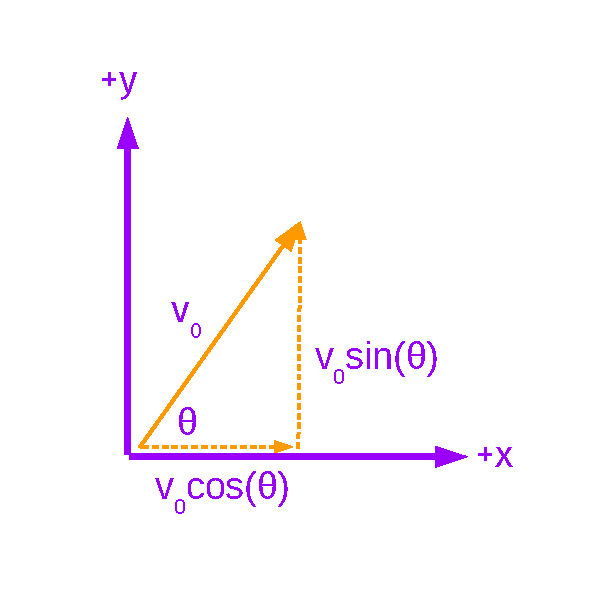
\includegraphics[width=0.5\textwidth,trim=1cm 1cm 1cm 1cm,clip=true]{figures/Vectors1.pdf}
\caption{\label{fig:components} The initial velocity $v_{\rm 0}$ is broken into components.}
\end{figure}
\end{frame}

\begin{frame}{Projectile Motion}
\small
During a fireworks display, a shell is shot into the air with an initial speed of 50 m/s, at an angle of 60$^{\circ}$ above horizontal.  The fuse is timed to ignite the shell just as it reaches its highest point above the ground.  Calculate the height at which the shell explodes.
\begin{itemize}
\item A: 190 m
\item B: 100 m
\item C: 110 m
\item D: 250 m
\end{itemize}
\end{frame}

\begin{frame}{Projectile Motion}
\small
How much time passes between the launch and the explosion?
\begin{itemize}
\item A: 3.9 seconds
\item B: 4.3 seconds
\item C: 5.1 seconds
\item D: 10.0 seconds
\end{itemize}
\end{frame}

\begin{frame}{Projectile Motion}
What is the horizontal displacement of the shell when it explodes?
\begin{itemize}
\item A: 108 meters
\item B: 98 meters
\item C: 98 degrees
\item D: 150 meters
\end{itemize}
\end{frame}

\begin{frame}{Projectile Motion}
\small
Let's try gaining visual intuition about projectile motion through the following program: \\
\vspace{0.25cm}
\url{http://galileoandeinstein.physics.virginia.edu/more_stuff/Applets/Projectile/projectile.html}\\
\begin{enumerate}
\item First, set air resistance to zero, at bottom right.
\item Make ten measurements of $g$ by creating some projectile trajectories, and taking the ratio $g = v_{\rm 0,y}^2/(2\Delta y)$.  What value do you obtain, on average?
\item Now, set air resistance to $b/m \approx 0.02$, and repeat the ten measurements.  What value do you obtain?
\item Explain why this value is smaller, larger, or equal to the first set of measurements.
\end{enumerate}
\end{frame}

\begin{frame}{Projectile Motion}
Projectile motion in two dimensions, with constant acceleration in one dimension, produces \textit{quadratic curves}.  How do we obtain the \alert{trajectory}, or $y(x)$ for these curves?  Looking at the x-direction:\\
\begin{align}
x &= v_{\rm 0}\cos(\theta) t \\
t &= \frac{x}{v_{\rm 0} \cos(\theta)} \label{eq:subst}
\end{align}
\end{frame}

\begin{frame}{Projectile Motion}
Substituting in Eq. \ref{eq:subst} for $t$ into the equation for vertical displacement gives:\\
\begin{align}
y(t) - y_{\rm 0} &= -\frac{1}{2}g\frac{x^2}{v_{\rm 0}^2\cos^2(\theta)} + \tan(\theta) x \\
y(t) - y_{\rm 0} &= -\left(\frac{g}{2v_{\rm 0}^2\cos^2(\theta)}\right)x^2 + \tan(\theta) x \\
y(x) &= -kx^2 + bx + y_{\rm 0}\label{eq:projfinal}
\end{align}
In Eq. \ref{eq:projfinal}, we are simply saying that $y(x)$ is some quadratic.  (It's still true that $y$ and $x$ are both functions of \textit{time}, however, those functions of time are related).
\end{frame}

\begin{frame}{Projectile Motion}
A space explorer is on a moon around another planet, and wants to measure $g$.  She tosses a pebble from an initial height of 2 meter, at an angle of 45 degrees above horizontal, with an initial velocity of 2 m/s.  When it lands, the horizontal displacement is 10 meters.  What is the gravitational acceleration $g$?
\begin{itemize}
\item A: 0.125 m/s$^2$
\item B: 0.25 m/s$^2$
\item C: 0.5 m/s$^2$
\item D: 1.0 m/s$^2$
\end{itemize}
\end{frame}

\begin{frame}{Projectile Motion}
Other useful equations are for the \textit{time-of-flight}, and the \textit{range}, concepts we've already seen in several examples: \\
\begin{align}
T_{\rm tof} &= \frac{2v_{\rm 0}\sin\theta}{g} \\
R &= \frac{v_{\rm 0}^2\sin2\theta}{g}
\end{align}
\end{frame}

\begin{frame}{Projectile Motion}
\alert{Algebraic challenge}: Show that the ratio of the range to the time is just the horizontal velocity, using the trigonometric identity $\sin(2\theta) = 2\sin\theta\cos\theta$.
\end{frame}

\section{Relative Motion and Addition of Velocities}

\begin{frame}{Relative Motion and Addition of Velocities}
Thus far, we have been discussing \textit{kinematics} with respect to a \textit{fixed frame of reference}.  Usually, we think of this frame of reference as the Earth.  If we kick a soccer ball, we know how to use equations to describe the motion.  What if we are moving, and the ball is moving with us, when we kick it?
\end{frame}

\begin{frame}{Relative Motion and Addition of Velocities}
Michael is running at 5 m/s, with a soccer ball rolling with him at the same speed.  He shoots the ball, such that he judges the speed to be 10 m/s.  What is the speed of the ball for someone who is observing, and standing still?
\begin{itemize}
\item A: 5 m/s
\item B: 10 m/s
\item C: 15 m/s
\item D: Cannot determine.
\end{itemize}
\end{frame}

\begin{frame}{Relative Motion and Addition of Velocities}
\begin{figure}
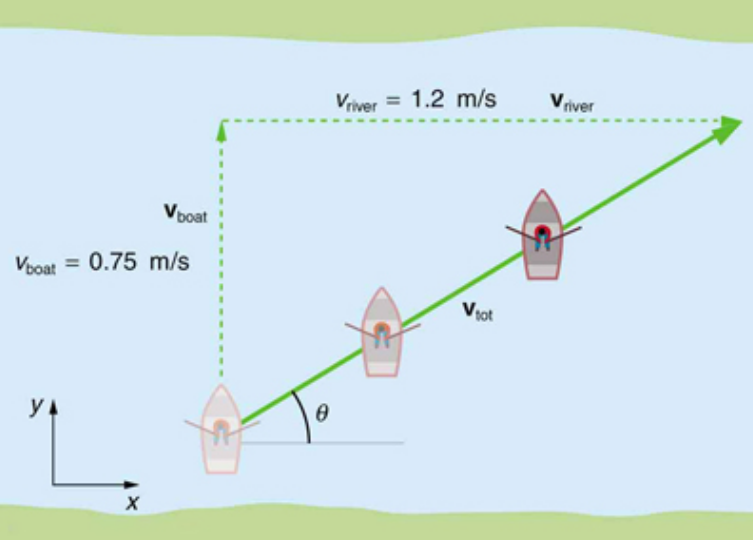
\includegraphics[width=0.6\textwidth]{figures/relative.png}
\caption{\label{fig:rel} Motion with respect to the ground requires the addition of the velocity of the river and the boat.}
\end{figure}
\end{frame}

\begin{frame}{Relative Motion and Reference Frames}
\small 
\textbf{The old train-robber problem:} a robber is riding a horse alongside a train moving in the $\hat{j}$ direction, at 5 m/s initially.  The robber on on the $-\hat{i}$ side of the train, and angles his run at 30 degrees with respect to the $\hat{j}$ direction toward the train.  His horse runs at a speed of 6 m/s.  What is the horse and robber's velocity, relative to the train?\\
\begin{itemize}
\item A: $3\hat{i}$ m/s
\item B: $\sqrt{2}\hat{i} + \sqrt{2}\hat{j}$ m/s
\item C: $(3\sqrt{3}-5)\hat{i} + 3\hat{j}$  m/s
\item D: $3\hat{i} + (3\sqrt{3}-5)\hat{j}$  m/s
\end{itemize}
\end{frame}

\begin{frame}{Relative Motion and Reference Frames}
\small 
\textbf{The old train-robber problem:} The conductor realizes the robber is there!  When the robber is 6 m away from the train, the conductor accelerates by 1 m/s$^2$.  What is the train's speed along the track \textit{relative to the robber} when the robber reaches the train? (Check: is this faster or slower than what it was initially?)\\
\begin{itemize}
\item A: $7-3\sqrt{3}$ m/s
\item B: $5-3\sqrt{3}$ m/s
\item C: $3\sqrt{3}$  m/s
\item D: $\sqrt{3}$  m/s
\end{itemize}
\end{frame}

\begin{frame}{Relative Motion and Reference Frames}
\small 
\textbf{The old train-robber problem:} The conductor sees that the horse no longer has a rider, and assumes the robber made it onto the train.  He holds on tight, and pulls the emergency brake.  The ensuing deceleration is -3 m/s$^2$ from an initial train speed of 10 m/s.  At this moment the robber is dropping down from the hatch to the car carrying the gold bars.  The drop takes 0.5 seconds.  What is the horizontal velocity of the bars relative to the robber just before she lands?\\
\begin{itemize}
\item A: $-7$ m/s
\item B: $-1.5$ m/s
\item C: $7$  m/s
\item D: $10$  m/s
\end{itemize}
\end{frame}

\begin{frame}{Relative Motion and Reference Frames}
\small 
The robber tumbles, but reaches her feet and pounces on the gold, and begins to load gold into her pack.  The conductor, however, accelerates from 8 m/s at a rate of 1 m/s$^2$, to more quickly reach a tunnel 0.5 km ahead.  How much time does the robber have to load gold before the train reaches the tunnel?  What would be her velocity relative to the ground if she dropped vertically out of the train at that time? \\
\begin{itemize}
\item A: 20 s, 10 m/s
\item B: 25 s, 15 m/s
\item C: 31 s, 17 m/s
\item D: 25 s, 33 m/s
\end{itemize}
\end{frame}

\begin{frame}{Relative Motion and Reference Frames}
\small 
\textbf{The old train-robber problem:} Looking ahead from the train, the robber realizes she cannot jump without hitting the tunnel wall.  The conductor opens the door with a pistol aimed, and shouts ``Hands up!''  The robber concludes which of the following?  \\
\begin{itemize}
\item A: Crime doesn't pay
\item B: Studying physics helps robbers commit crimes more efficiently
\item C: She should have gone into a career in science
\item D: Gold is heavy
\end{itemize}
\end{frame}

\begin{frame}{Relative Motion and Reference Frames}
\small
Relative velocities is also a good model for the difference between ``air-speed'' and ``ground-speed.''  Suppose a plane can fly at 100 kph in still air, but experiences a tailwind of 20 kph.  What is the ``ground-speed'' of the aircraft?
\begin{itemize}
\item A: 80 kph
\item B: 120 kph
\item C: 100 kph
\item D: 20 kph
\end{itemize}
\end{frame}

\begin{frame}{Relative Motion and Reference Frames}
\small
Suppose the wind changes.  The plane is traveling due East ($\hat{i}$ direction), and the wind moves towards Northeast (45 degrees with respect to East), and has a new speed of 40 kph.  What is the ground speed of the aircraft?
\begin{itemize}
\item A: $100\hat{i} + 40/\sqrt{2}\hat{j}$  kph
\item B: $(100+40/\sqrt{2})\hat{i} + 40/\sqrt{2}\hat{j}$  kph
\item C: $40/\sqrt{2}\hat{i} + 40/\sqrt{2}\hat{j}$  kph
\item D: $(100+40/\sqrt{2})\hat{i}$  kph
\end{itemize}
\end{frame}

\section{Conclusion}

\begin{frame}{Week 3 Summary}
\begin{enumerate}
\item Working with vectors: displacement, velocity and acceleration
\begin{itemize}
\item Breaking into components, graphical methods
\item Analytical methods
\item \textbf{Lab-activity: measuring different accelerations}
\item \textbf{Lab-activity: testing component independence}
\end{itemize}
\item Combining free-fall and vector components: \alert{projectile motion}
\item Relative motion and addition of velocities
\end{enumerate}
\end{frame}

\section{Answers}

\begin{frame}{Answers}
\begin{columns}[T]
\begin{column}{0.5\textwidth}
\begin{itemize}
\item To the right, positive
\item At the peak height, yes, no
\item $\vec{r}_{\rm final} = 450.0 \hat{i} + 80.0\hat{j}\quad (m)$
\item $\vec{v}_{\rm final} = 6.5 \hat{i} + 1.2\hat{j}\quad (m/s)$
\item $20/3$ ns
\item 6\%
\item $(2.45)\hat{i}-(0.38)\hat{j} \quad (m/s)$
\item $-3\hat{i}$
\item 3.45 m/s, 3.94 m/s
\item (3.19,1.32) m/s
\item (1.22,3.75)
\end{itemize}
\end{column}
\begin{column}{0.5\textwidth}
\begin{itemize}
\item 100 m
\item 4.3 s
\item 108 m
\item 0.5 m/s$^2$ 
\item $3\hat{i} + (3\sqrt{3}-5)\hat{j}$ m/s
\item $7-3\sqrt{3}$ m/s
\item $-1.5$ m/s
\item 25 s, 33 m/s
\item Gold is heavy...jokes
\item 120 kph
\item $(100+40/\sqrt{2})\hat{i} + 40/\sqrt{2}\hat{j}$  kph
\end{itemize}
\end{column}
\end{columns}
\end{frame}

\end{document}
